\documentclass{article}
\usepackage[utf8]{inputenc}

% Basic packages
	\usepackage{amssymb}
	\usepackage{amsmath}
	\usepackage{graphicx}
	\usepackage[english]{babel}
	\usepackage{natbib}

% Relevant packages
	\usepackage{bm}
	\usepackage{bbm}
	\usepackage{geometry}
	\usepackage{enumitem}
	\usepackage{listings}

% Document settings
	\geometry{a4paper,margin=15mm}

	\setlist[itemize]{nolistsep,noitemsep}
		
	\setlength{\parindent}{0pt}
	\setlength{\parskip}{1.5em}
	\renewcommand{\baselinestretch}{1.2}

	\setlength{\abovedisplayskip}{1.2em}
	\setlength{\belowdisplayskip}{1.2em}
	\renewcommand{\arraystretch}{1.2}

\begin{document}
	\section{pohybová rovnice diskretizované soustavy}
	``\emph{Zapište pohybovou rovnici diskretizované soustavy (analogicky rovnici rovnováhy ze statiky ve tvaru $\bm{K}\bm{U} = \bm{F}$. Vysvětlete význam jednotlivých členů.}''

	\begin{equation}
		\bm{M}\bm{\ddot{\delta}} + \bm{C}\bm{\dot{\delta}} + \bm{K}\bm{\delta} - \bm{F} = \bm{0}
	\end{equation}
	\begin{itemize}
		\item [$\bm{\delta}$] - vektor uzlových posuvů
		\item [$\bm{M}$] - matice hmotnosti
		\item [$\bm{C}$] - matice tlumení
		\item [$\bm{K}$] - matice tuhosti
		\item [$\bm{F}$] - vektor vnějších sil
	\end{itemize}

	\section{diferenční operátor}
	\emph{``Vysvětlete pojem \textbf{diferenční operátor} (diferenční schéma). Jako příklad navrhněte diferenční schéma pro diferenciální operátory $\frac{d\bm{U}}{dt},\frac{d^2\bm{U}}{dt^2}$.''}

	Diferenční operátor je takový operátor, kterým dokážeme aproximovat derivaci funkce v daném bodě pomocí hodnot funkce v jeho okolí (moje definice).
	
	Vychází z taylorova rozvoje
	\begin{equation}
		\bm{U}(t_0+\Delta t) \approx \bm{U}(t_0) + \frac{d\bm{U}(t_0)}{dt} \Delta t + \frac{1}{2} \frac{d^2\bm{U}(t_0)}{dt^2} \Delta t^2 + \dots
	\end{equation}
	kde první derivaci lze tímpádem aproximovat jako
	\begin{equation}
		\frac{d\bm{U}(t_0)}{dt} \approx \frac{\bm{U}(t_0+\Delta t) - \bm{U}(t_0)}{\Delta t}
	\end{equation}

	\textbf{Dopředná diference prvního řádu}
	\begin{equation}
		\frac{d\bm{U}_{t_0^+}}{dt} = \frac{\bm{U}_{t_0+\Delta t} - \bm{U}_{t_0}}{\Delta t}
	\end{equation}

	\textbf{Zpětná diference prvního řádu}
	\begin{equation}
		\frac{d\bm{U}_{t_0^-}}{dt} = \frac{\bm{U}_{t_0} - \bm{U}_{t_0-\Delta t}}{\Delta t}
	\end{equation}

	\textbf{Centrální diference druhého řádu}
	\begin{equation}
		\frac{d^2\bm{U}_{t_0}}{dt^2}
		=
		\frac{\frac{d\bm{U}_{t_0^+}}{dt} - \frac{d\bm{U}_{t_0^-}}{dt}}{\Delta t}
		=
		\frac{\bm{U}_{t_0+\Delta t} - 2\bm{U}_{t_0} + \bm{U}_{t_0-\Delta t}}{\Delta t^2}
	\end{equation}

	\section{Konzistence matice hmotnosti}
	\emph{``Vysvětlete pojmy konzistentní a nekonzistentní matice hmotnosti a vztah k explicitnímu integračnímu schématu. Jakou výhodu přináší užití nekonzistentní matice a za jakou cenu?''}

	Konzistentní matice hmotnosti vzniká sestavením z matic hmotnosti elementů ve tvaru $\bm{M}^e = \int_{(V_e)} \bm{N}^T \rho \, dV$ (konzistentním s energetickým přístupem), které obsahují i mimo diagonální prvky. Pak se rovnice netlumeného systému řeší rozkladem matice $\bm{M}$ do diagonálního tvaru.

	Existuje přístup ke konstrukci matice hmotnosti, který rozdělí hmotu elementu do uzlů (aproximace). Pak má matice hmotnosti systému (stejně jako jednotlivé matice elementů) pouze diagonální členy a názýváme ji nekonzistentní.

	\section{Modální transformace}
	\emph{``Definujte operátor (matici) modální transformace $\Phi$, popište jeho vlastnosti a naznačte transformaci rovnice (*) do modálních souřadnic.''}

	Je-li matice $\Phi$ řešením problému vlastních čísel
	\begin{equation}
		\bm{K}\bm{\Phi} = \bm{\Omega}^2 \bm{M} \bm{\Phi}
	\end{equation}
	kde $\bm{\phi}_i$ jsou vlastní vektory a $\omega_i$ vlastní frekvence tvořící matice $\bm{\Phi}$ a $\bm{\Omega}$  
	\begin{equation}
		\bm{\Phi} = \begin{bmatrix} \bm{\phi}_i & \dots & \bm{\phi}_N \end{bmatrix}
		\,,\;
		\bm{\Omega}^2 = \operatorname{diag}(\omega_i^2)
		\;,\quad 
		i \in \langle 1,N \rangle
	\end{equation}
	platí
	\begin{equation}
		\bm{\Phi}^T\bm{M}\bm{\Phi} = \bm{1}
		\;,\quad 
		\bm{\Phi}^T\bm{K}\bm{\Phi} = \bm{\Omega}^2
	\end{equation}

	Soustavu pohybovných rovnic systému s proporčním tlumením
	\begin{equation}
		\bm{M}\bm{\ddot{\delta}} + \bm{C}\bm{\dot{\delta}} + \bm{K}\bm{\delta} = \bm{F}
	\end{equation}
	lze zavedením modální souřadnice $\bm{q} = \bm{\Phi}\bm{\delta}$ a vynásobením transponovanou maticí modální transformace $\bm{\Phi}^T$ zleva, převést do tvaru
	\begin{equation}
		\bm{\ddot{q}} + \bm{\Gamma}\bm{\dot{q}} + \bm{\Omega}^2 \bm{q} = \bm{\Phi}^T \bm{F}
		\;,\quad 
		\bm{\Gamma} = \operatorname{diag}(2\,\omega_i\xi_i) \;,\quad i \in \langle 1,N \rangle
	\end{equation}
	kde $\xi_i$ jsou poměrné útlumy.

	Soustava se pak rozpadá na rovnice ve tvaru
	\begin{equation}
		\ddot{q}_i + 2\,\omega_i\xi_i \dot{q} + \omega_i^2 q = f_i
		\;,\quad 
		f_i = \bm{\phi}_i \cdot \bm{F}
		\;,\quad 
		i \in \langle 1,N \rangle
	\end{equation}

	\section{}
	\begin{equation}
		d\bm{x} = \bm{F} \, d\bm{X}
	\end{equation}
	přičemž $\bm{F}$ je regulární tzn. $\det(\bm{F}) > 0$ a dále platí
	\begin{equation}
	\bm{F} = \bm{1} + \bm{Z}
	\;,\quad 
	\bm{Z} = \frac{\partial \bm{u}}{\partial \bm{X}}
	\end{equation}

	\section{}
	\emph{``Popište princip Newton–Raphsonova iteračního schématu v přírůstkové metodě. Využijte grafické znázornění pro jeden stupeň volnosti a pro soustavu s mnoha stupni volnosti naznačte vývojový diagram.''}
	\begin{enumerate}
		\item $\bm{u} = \bm{u}_0$
		\item 	$\bm{F}^I = \bm{K}_T(\bm{u})\,\bm{u}$
		\item $\bm{F}^N = \bm{F}^E - \bm{F}^I$
		\item $\|\bm{F}^N\| < \varepsilon$ \textbf{?} return \textbf{:} nothing
		\item $\Delta \bm{u} = \bm{K}_T(\bm{u})^{-1} \bm{F}^N$
		\item $\bm{u} = \bm{u} + \Delta \bm{u}$
		\item zpět na 2.
	\end{enumerate}
	\begin{figure}
		\centering
		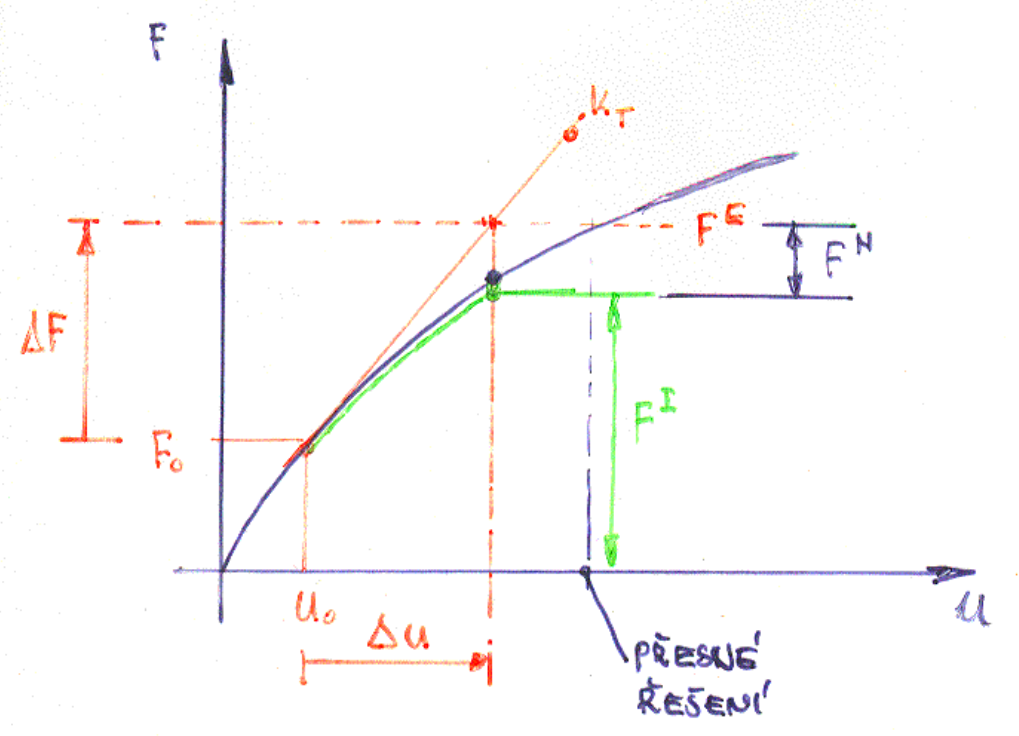
\includegraphics[width=.5\linewidth]{NR1.png}
	\end{figure}
	\begin{figure}
		\centering
		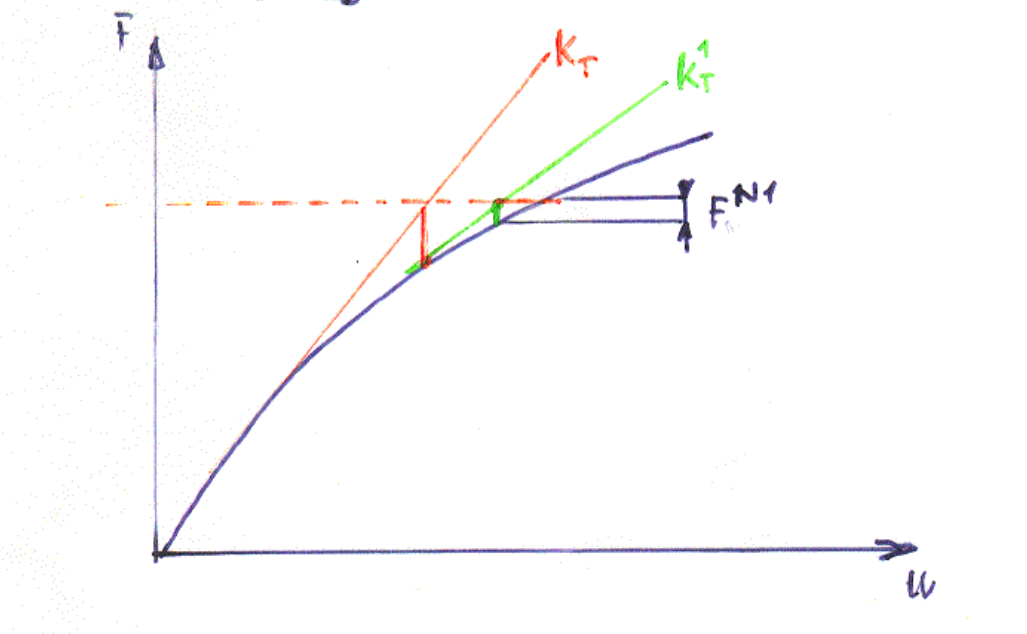
\includegraphics[width=.5\linewidth]{NR2.png}
	\end{figure}
\end{document}